\section{Data Sources and Reduction}
\label{sec:data}
\subsection{Data Sources}
In order to analyze the physical distribution of \agb\, stars in the IR, we require reliable identifications of known \agb, stars to generate color-color selection criteria. We select \agb\, stars from three source catalogs: the {\it Optical Gravitational Lens Experiment-III Variable Star Catalog} \citep[\ogle,][]{2008AcA....58...69U,2009AcA....59..239S,2011AcA....61..217S}, the {\it MAssive Compact Halo Objects} project \citep[\macho,][]{1997ApJ...482...89A}, and the \simbad\, Astronomical Database \citep{2000A&AS..143....9W}. \ogle\, photometry for Long-Period Variables (LPVs) in the Small and Large Magellanic Clouds (SMC and LMC respsectively) was obtained between July 2001 and May 2009, with stars in the central 4.5-deg$^2$ of the LMC and SMC having an additional 5 observing seasons of photometry from OGLE-II. O-rich and C-rich \agb\, stars in \ogle\, were photometrically selected using reddening-free Wesenheit magnitudes, described in \cite{2009AcA....59..239S,2011AcA....61..217S}. Data reduction techniques are described in \cite{2008AcA....58...69U}. The resulting samples yielded 46,467 \agb\, stars from the LMC (37,203 O-rich; 9,264 C-rich) and 6,509 stars from the SMC (3,727 O-rich; 2,782 C-rich). From \macho\, we obtain the sample of SMC, LMC, and Galactic Bulge AGB stars used in \cite{2008AJ....136.1242F} (14,861 stars). The sample of AGB stars from \simbad\, was obtained by querying for all objects classified as C-stars (18,656), S-stars (1,108), OH/IR stars (825), AGB stars (2,359), and Mira variables (9,608), for a total of 32,556 stars. The total sample of \agb\, stars is 100,393.

Since \sdss\, is an optical survey of unprecedented extent and sensitivity, we use \sdss\, spectroscopic catalogs to select contaminant sources for the NIR-MIR color-color fields of \agb\, stars. Data for active galactic nuclei (AGN; 19,184 objects), quasi-stellar objects (QSOs; 122,550 objects), and star forming/burst galaxies (820,272 objects total) were drawn from \sdss\, DR7, specifically from the NYU Value Added Galaxy Catalog\footnote{\url{http://sdss.physics.nyu.edu/vagc/}} \citep[VAGC]{2005AJ....129.2562B}. Luminous Red Galaxies (LRGs) were selected from the SDSS Luminous Red Galaxy Survey \citep[105,631 objects, ][]{2010ApJ...710.1444K}.  Data for stars in the SDSS stellar locus were drawn from the DR 9 SEGUE Stellar Parameters Pipeline (SSPP) \citep[1,843,190 objects, ][]{2012ApJS..203...21A}.

In this study, we rely heavily on data from the \allwise\, extension of the \wise\, survey, combining data from the initial All-Sky Data Release, the 3-band cryogenic data release, and the NEOWISE post-cryogenic data release \citep{2013wise.rept....1C}. The initial \wise All-Sky Data Release observed the sky between January and August 2010, observing the sky 1.2 times with four detectors, operating at 3.4, 4.6, 12, and 22$\mu$m. Hereon we refer to \allwise\, photometric bands at [3.4$\mu$m/4.6$\mu$m/12$\mu$m/22$\mu$m] as [$W1/W2/W3/W4$]. The positions of objects in the \wise\, catalog were calibrated to the \twomass\, point source catalog. The 3-band cryogenic data release contains data from $W1$, 2, and 3, and surveyed $30\%$ of the sky between August and October 2010. During the 3-band cryogenic survey, $W1$ and $W2$ operated with nearly the same sensitivity as during the full survey. Warming of the telescope reduced sensitivty in $W3$ and fully saturated $W4$. The NEOWISE post-cryogenic data release contains $W1$ and $W2$ measurements, with sensitivities close to those obtained during the full cryogenic phase. During this phase, \wise\, surveyed $70\%$ of the sky. Data products from the post-cryogenic release included updated instrumental, astrometric, and photometric calibrations and reduction algorithms, resulting in much lower SNR. The overall total number of sources compiled into \allwise\, totals over 747.6 million.

\subsection{Data Reduction}
We use NASA/IPAC IRSA's {\tt GATOR} tool\footnote{\url{http://irsa.ipac.caltech.edu/cgi-bin/Gator/nph-scan?mission=irsa&submit=Select&projshort=WISE}} to positionally match \sdss, \ogle, \macho, and \simbad\, to \allwise. We select only matches within 3" between our main sample of known \agb\, stars and \allwise. All samples of \agb\, star matches were required to be brighter than the published 5$\sigma$ faint limits of [16.83/15.6/11.32/8.0], as well as fainter than the saturation limits of [2.0/1.5/-3.0/-4.0] extrapolated from the wings of the PSFs for point sources, for [$W1/W2/W3/W4$] \citep{2013wise.rept....1C}, with no confusion or contamination flags in [$W1/W2/W3/W4$]. We require only single associations with \twomass\, objects within 3", detections in \twomass\, $J$, $K_s$, and all \allwise\, magnitudes as well as SNR $>$ 3 in each \allwise\, band. 
%We do not enforce the same faint or saturation limits on our contaminant samples. As a show of the strength of our selection criteria, we seek to include matches to each contaminant with reasonable detections in \allwise, and magnitudes reliable enough to perform the necessary color selections. We limit our sample from the \sdss\, DR9 SSPP to objects within 0.5 dex of the $g'-r'$ vs. $g'-i'$ stellar locus \citep{2014MNRAS.440.3430D}, \sdss\, SNR $>$ 5, [$W1/W2/W3/W4$] SNR $>$ 3,  detections in \twomass\, $J$ and $K_s$ bands, and one 2MASS association within 3". Objects from the NYU VAGC were reduced with requirements of SNR $>$ 3 for [$W1/W2/W3/W4$], required detections for \twomass\, $J$ and $K_s$ bands, and one \twomass\, association within 3". LRGs were required to have SNR $>$ 3 for [$W1/W2/W3$], detections for \twomass\, $J$ and $K_s$ bands, and one \twomass\, association within 3".  The restriction on $W4$ was dropped here, as it reduces the population of LRGs by an order of magnitude. 
The population for each sample from initial matching as well as after the application of the \allwise\, faint limits, saturation limits, and \twomass\, detection requirements are shown in Table~\ref{tab:pop}. The WISE color-color distributions for the AGB and contaminant samples are shown in Figure~\ref{fig:distros}. \\

\vspace{-10pt}
%\begin{table}[h]
%	\begin{center}
%	\caption{AGB and Contaminant Populations}
%	\scalebox{0.85}{\begin{tabular}{l c c c c c c}
%		\hline
%		Population & SIMBAD C stars & OH/IR stars & Miras & S stars & AGB stars \\
%		\hline
%		2" match & 13,245 & 294 & 8,850 & 1,078 & 1,665 \\
%		Reduced & 3,327 & 165 & 6,218 & 865 & 1,121 \\
%		\hline\hline
%		Population & MACHO seq1 & seq2 & seq3 & seq4\\
%		\hline
%		2" match & 5,193 & 3,441 & 2,548 & 2,931 \\
%		Reduced & 927 & 642 & 263 & 336 \\
%		\hline\hline
%		Population & OGLE C-rich & O-rich\\
%		\hline
%		2" match & 11,417 & 38,369 \\
%		Reduced & 737 & 2515 \\
%		\hline\hline
%		Population & Locus Stars & AGN & LRG & QSO & Galaxies \\
%		\hline
%		2" match & 1,508,158 & 18,481 & 102,178 &  & 799,761 \\
%		Reduced & 168,045 & 9,652 & 7,717 & 18,360 & 125,869 \\
%		\hline
%
%		\label{tab:pop}
%	\end{tabular}}
%	\end{center}
%\end{table}

\begin{table}[h]
	\begin{center}
	\caption{AGB and Contaminant Populations}
	\scalebox{0.85}{\begin{tabular}{l c c c c c c}
		\hline\hline
		Population & SIMBAD AGB* & C* & Mira & OH/IR & S* \\ 
		\hline
		3" match & 1,689 & 14,209 & 9,027 & 406 & 1,081 \\
		Reduced & 684 & 1,782 & 3,241 & 43 & 511 \\ 
		\hline
		Population & MACHO seq1 & seq2 & seq3 & seq4 \\ 
		\hline
		3" match & 5,279 & 3,519 & 2,619 & 3,070 \\
		Reduced & 277 & 185 & 73 & 61 \\ 
		\hline
		Population & OGLE-III C-rich & O-rich \\ 
		\hline
		3" match & 11,542 & 38,848 \\
		Reduced & 249 & 730 \\ 
		\hline
		Population & DR12 SSPP & DR7 LRG & QSO & AGN & Galaxies \\ 
		\hline
		3" match & 1,578,329 & 104,345 & 103,590 & 18,528 & 841,712 \\ 
		Reduced & 67,508 & 84 & 3,977 & 1,069 & 44,314 \\ 
		\hline\hline

		\label{tab:pop}
	\end{tabular}}    
	\end{center}
\end{table}

\begin{figure}
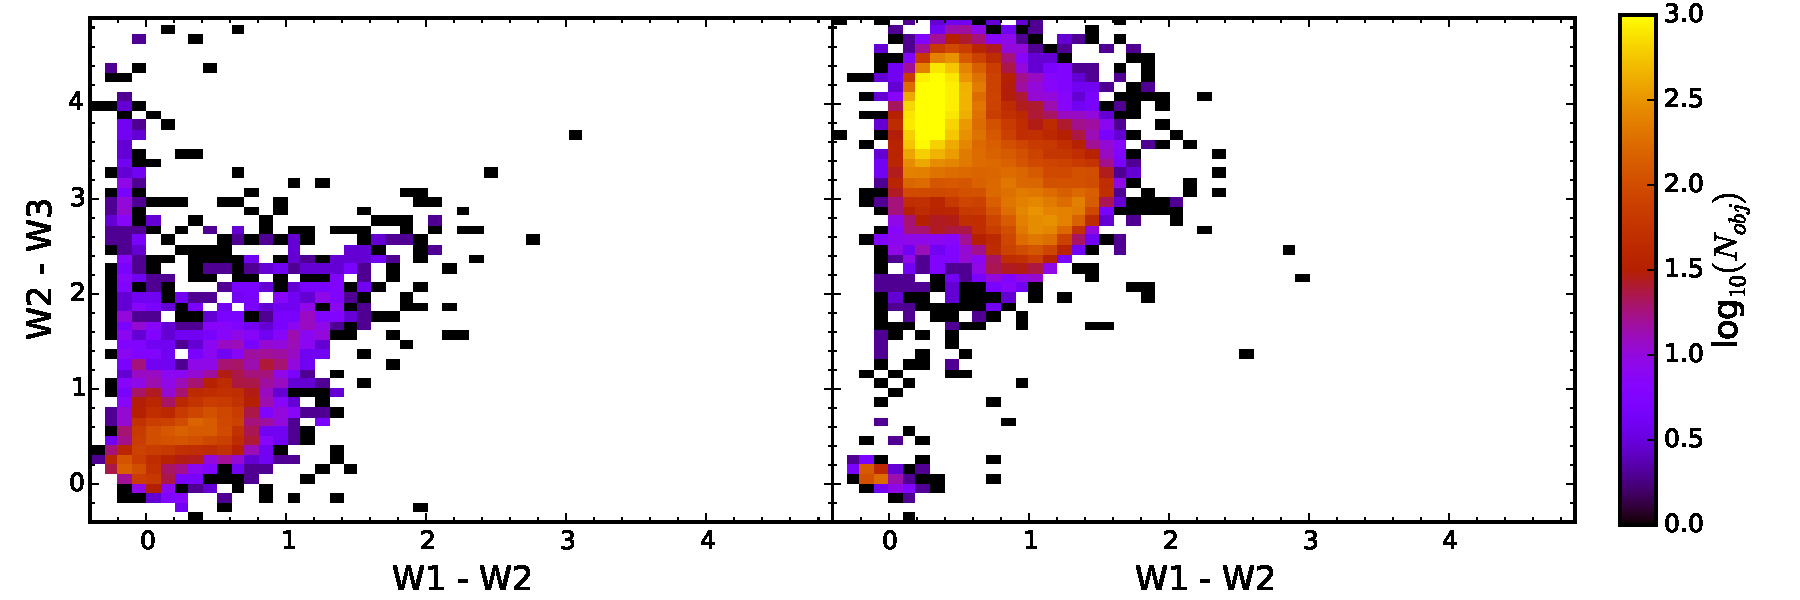
\includegraphics[width=7in]{figs/agbs_contaminants_color_color1.pdf}
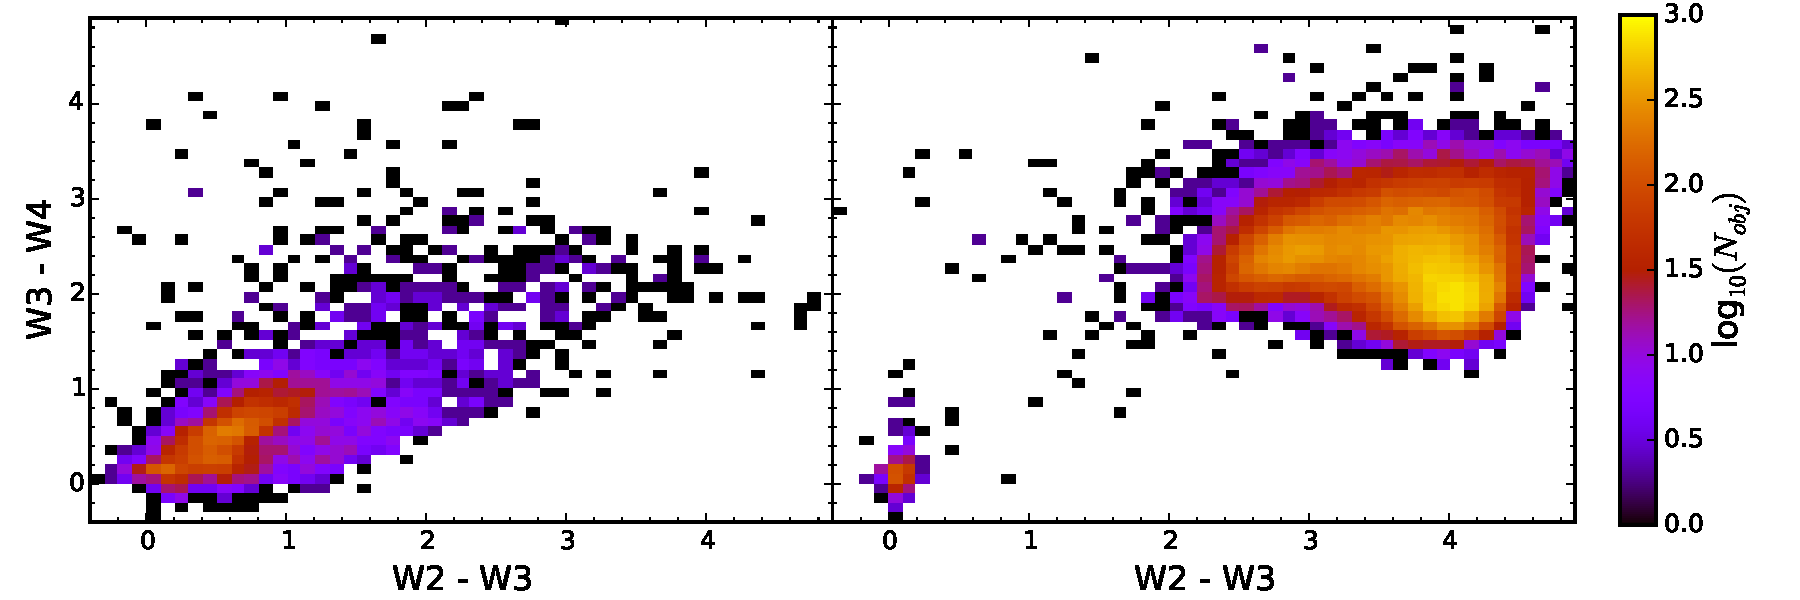
\includegraphics[width=7in]{figs/agbs_contaminants_color_color2.pdf}
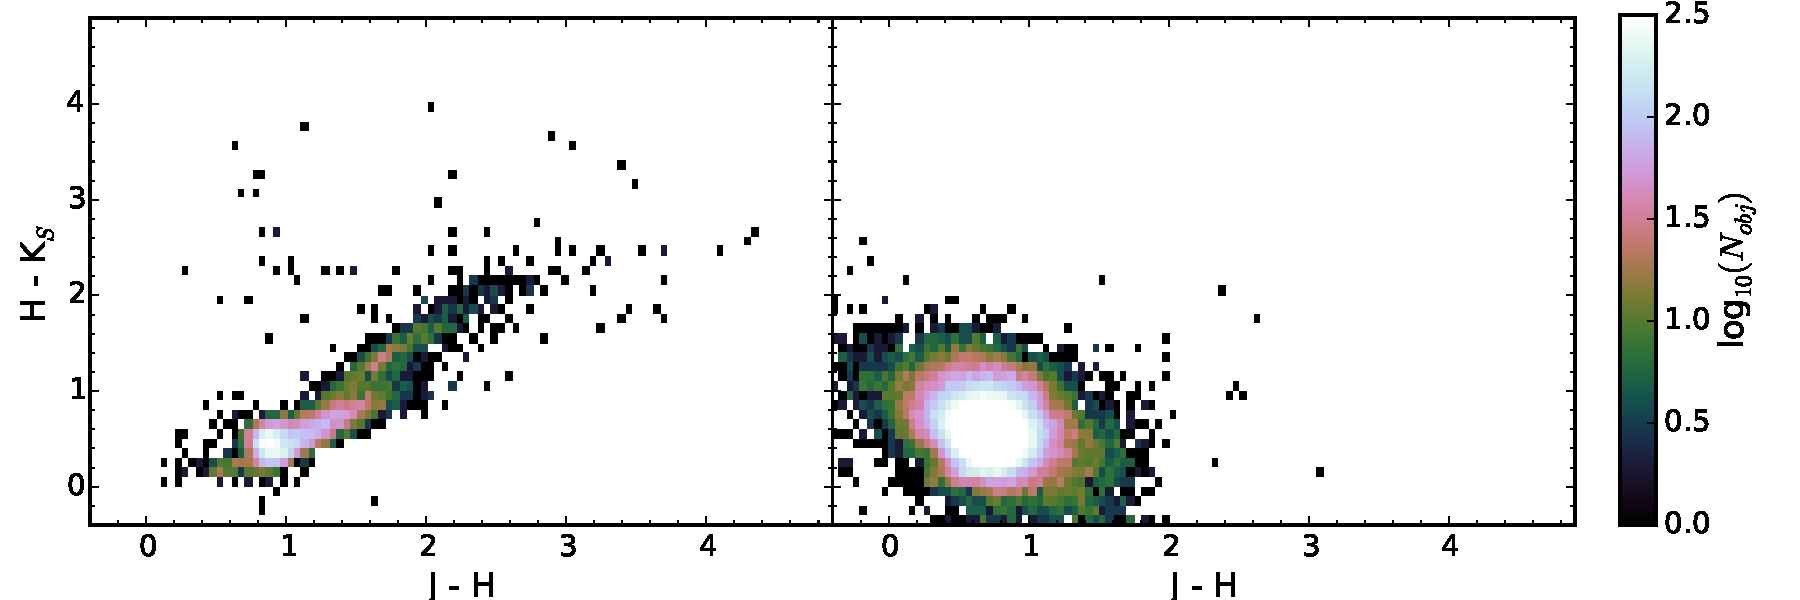
\includegraphics[width=7in]{figs/agbs_contaminants_color_color3.pdf}
\caption{\emph{Left:} Known AGB stars after data reduction. \emph{Right:} All contaminants after data reduction.\label{fig:distros}}
\end{figure}

